\documentclass[11pt,a4paper]{article}
\usepackage{graphicx}
\usepackage{caption}
\usepackage{longtable}
\usepackage{geometry}
\geometry{margin=1in}
\begin{document}
\begin{center}\huge\textbf{Linear Prediction Analysis for five vowels (/a/, /i/, /u/, /e/, /o/)}\end{center}
\vspace{1em}
\section*{Data used}
\textbf{File:} aeiou.wav (sample rate: 8000 Hz)\\ 
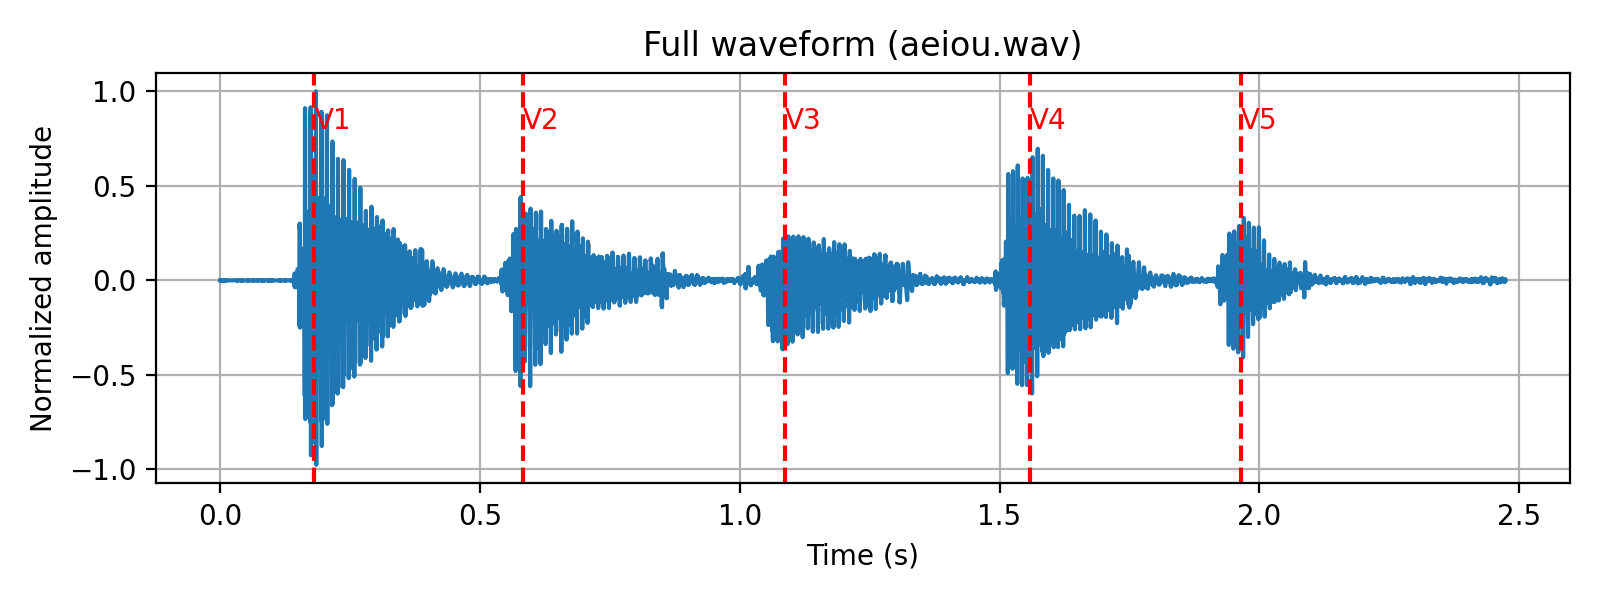
\includegraphics[width=\textwidth]{vowel_report_images/waveform_full.png}\\
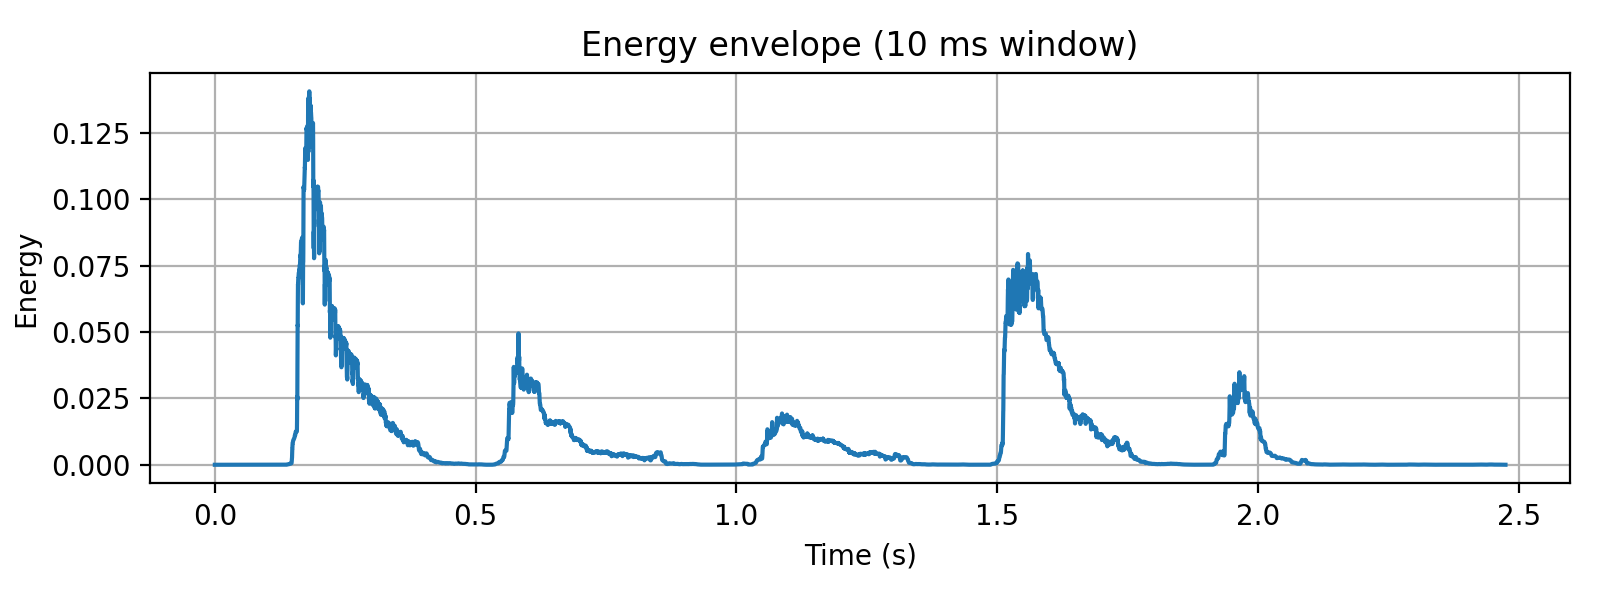
\includegraphics[width=\textwidth]{vowel_report_images/energy_env.png}\\
\section*{1. Recording / Data}
The audio file was inspected and five high-energy vowel segments were detected. The centers (sample indices) are listed below:
\begin{verbatim}
Vowel 1: center=1449 samples  (0.181 s)
Vowel 2: center=4657 samples  (0.582 s)
Vowel 3: center=8699 samples  (1.087 s)
Vowel 4: center=12472 samples  (1.559 s)
Vowel 5: center=15714 samples  (1.964 s)
\end{verbatim}
\section*{2. Time signals and pitch (F$_0$)}
\subsection*{Vowel 1}
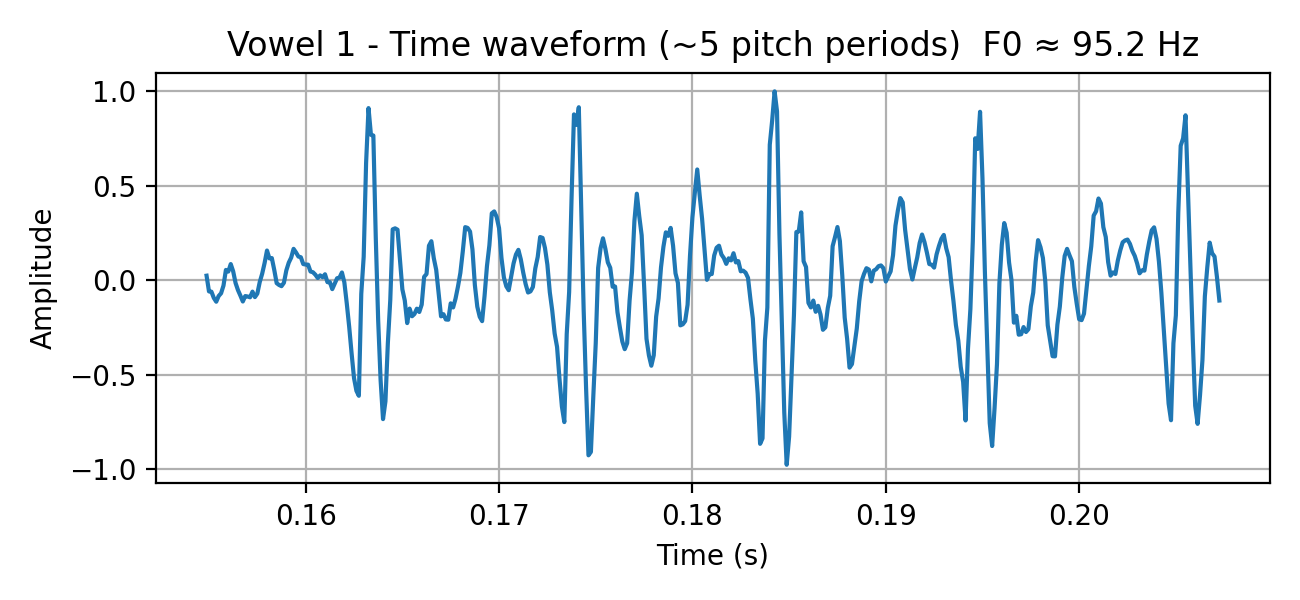
\includegraphics[width=0.9\textwidth]{vowel_report_images/vowel1_time.png}
\par Estimated F$_0$: 95.2 Hz\\ 
\subsection*{Vowel 2}
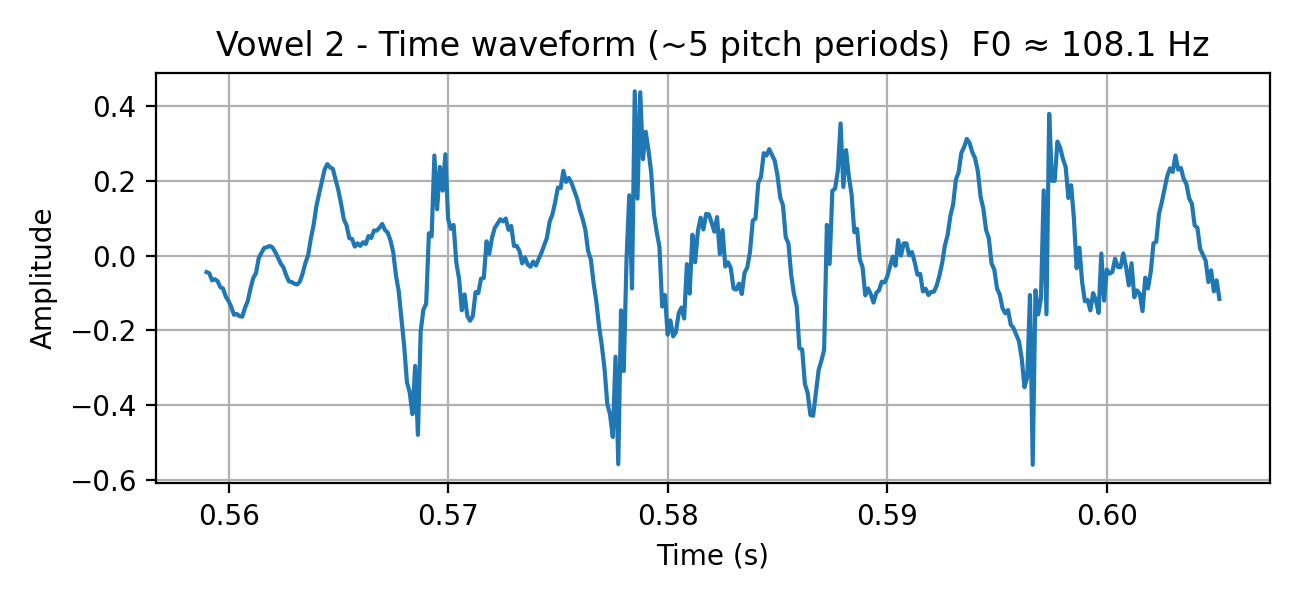
\includegraphics[width=0.9\textwidth]{vowel_report_images/vowel2_time.png}
\par Estimated F$_0$: 108.1 Hz\\ 
\subsection*{Vowel 3}
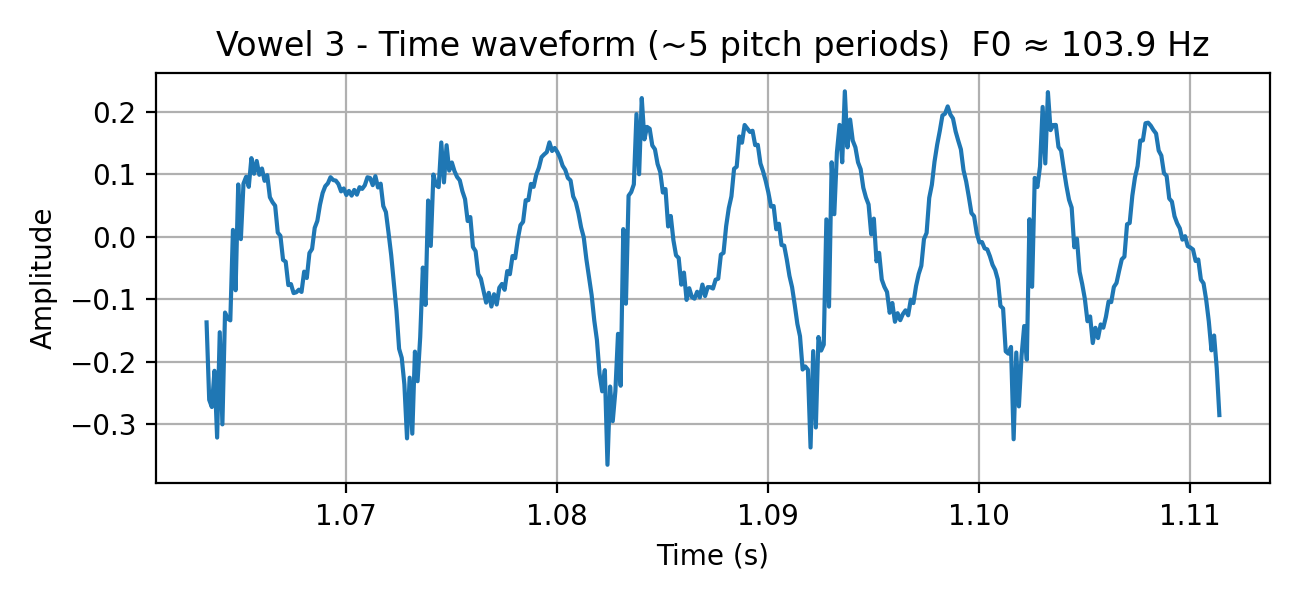
\includegraphics[width=0.9\textwidth]{vowel_report_images/vowel3_time.png}
\par Estimated F$_0$: 103.9 Hz\\ 
\subsection*{Vowel 4}
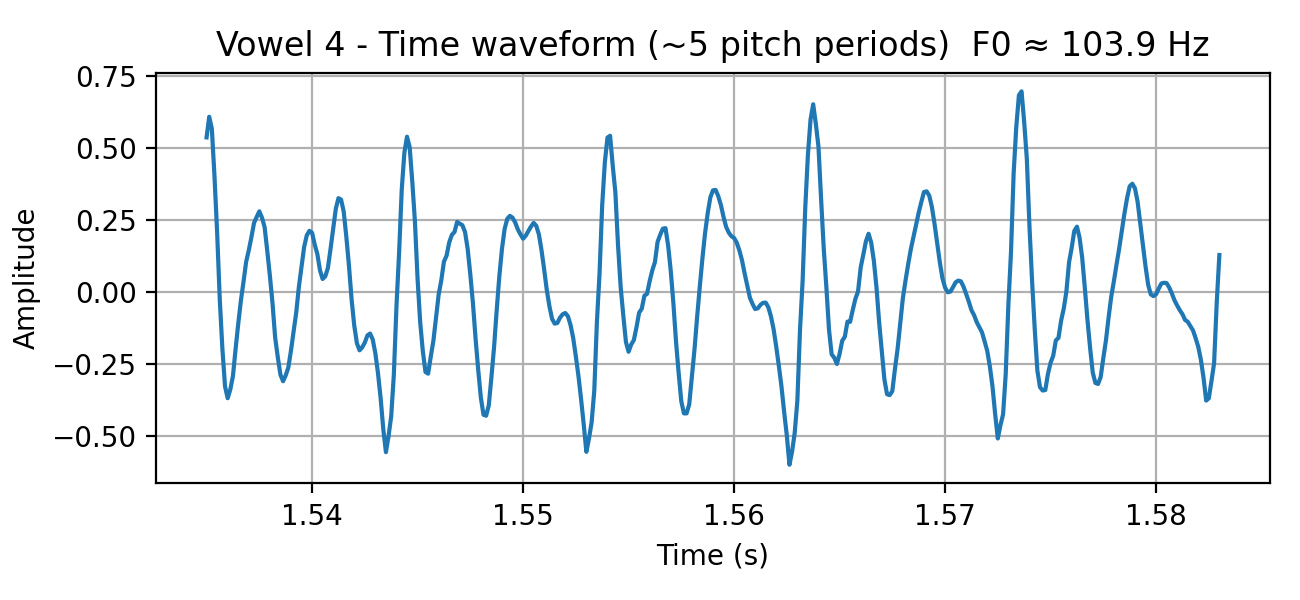
\includegraphics[width=0.9\textwidth]{vowel_report_images/vowel4_time.png}
\par Estimated F$_0$: 103.9 Hz\\ 
\subsection*{Vowel 5}
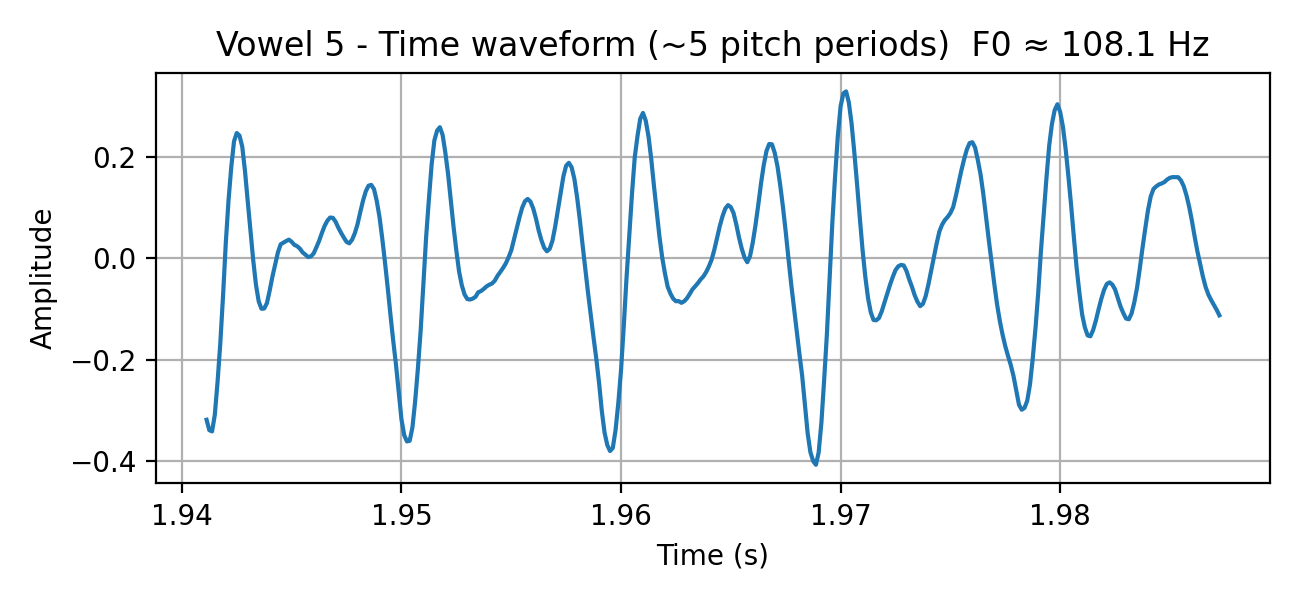
\includegraphics[width=0.9\textwidth]{vowel_report_images/vowel5_time.png}
\par Estimated F$_0$: 108.1 Hz\\ 
\section*{3. FFT power spectra (per vowel)}
\subsection*{Vowel 1}
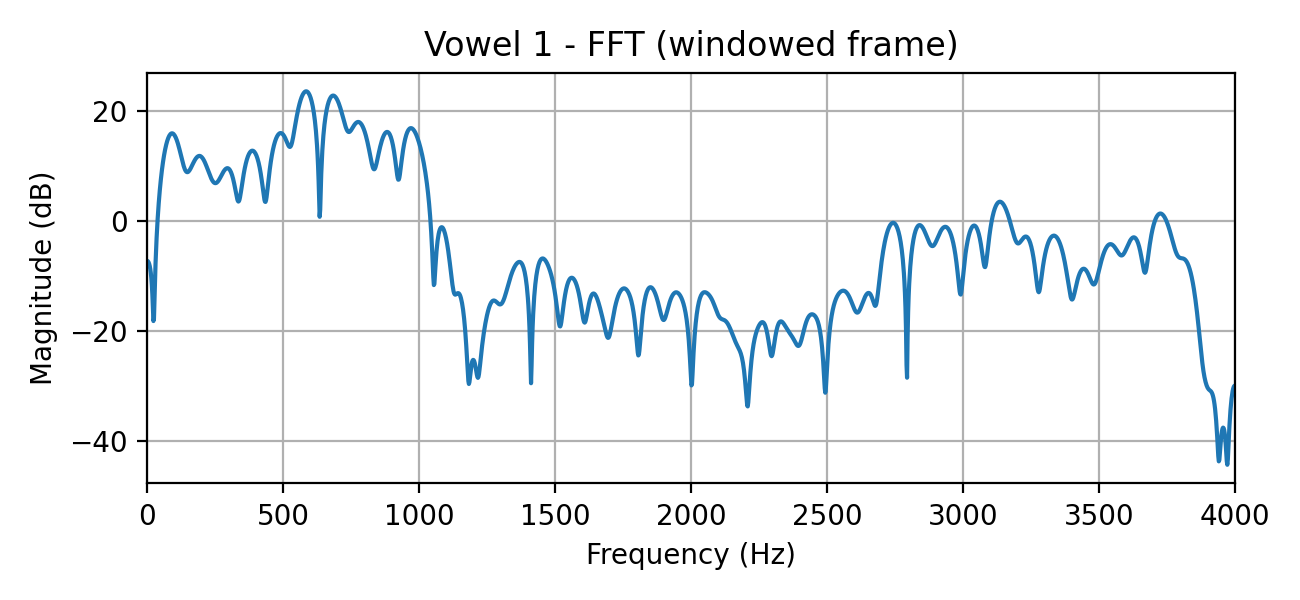
\includegraphics[width=0.9\textwidth]{vowel_report_images/vowel1_fft.png}
\subsection*{Vowel 2}
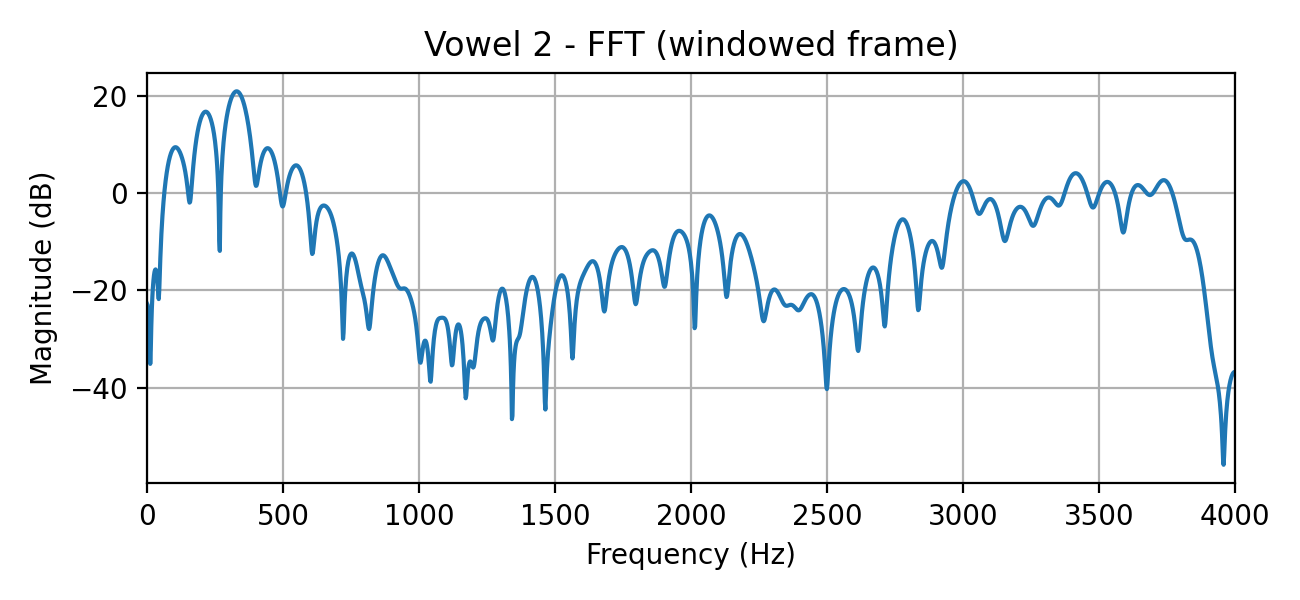
\includegraphics[width=0.9\textwidth]{vowel_report_images/vowel2_fft.png}
\subsection*{Vowel 3}
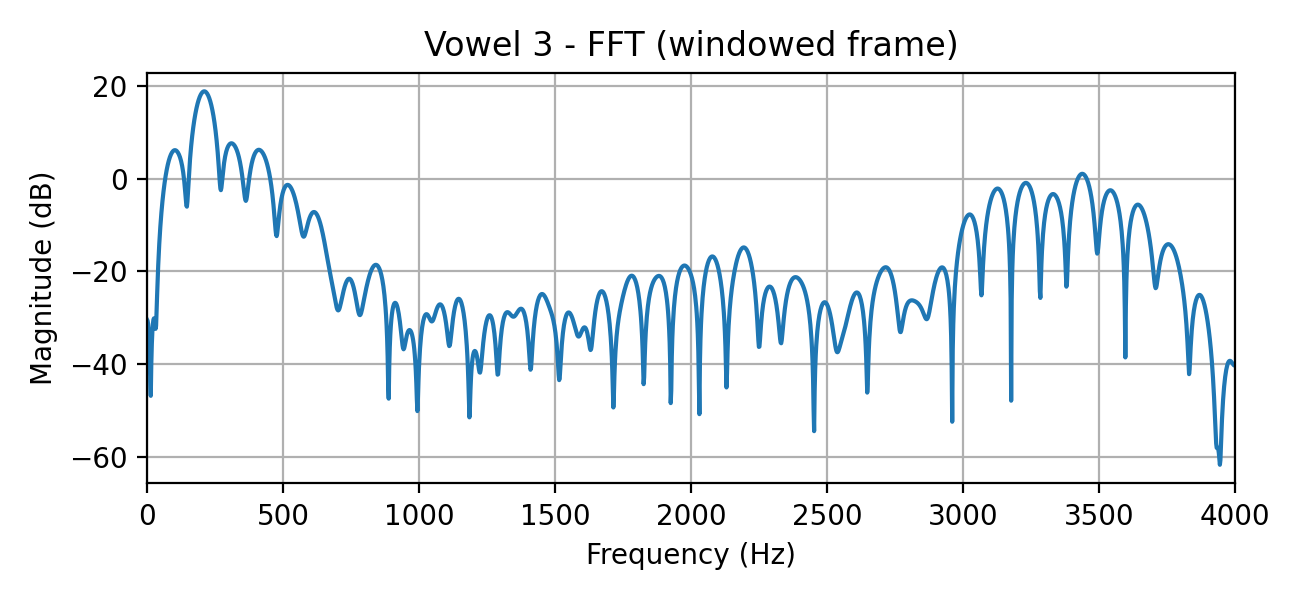
\includegraphics[width=0.9\textwidth]{vowel_report_images/vowel3_fft.png}
\subsection*{Vowel 4}
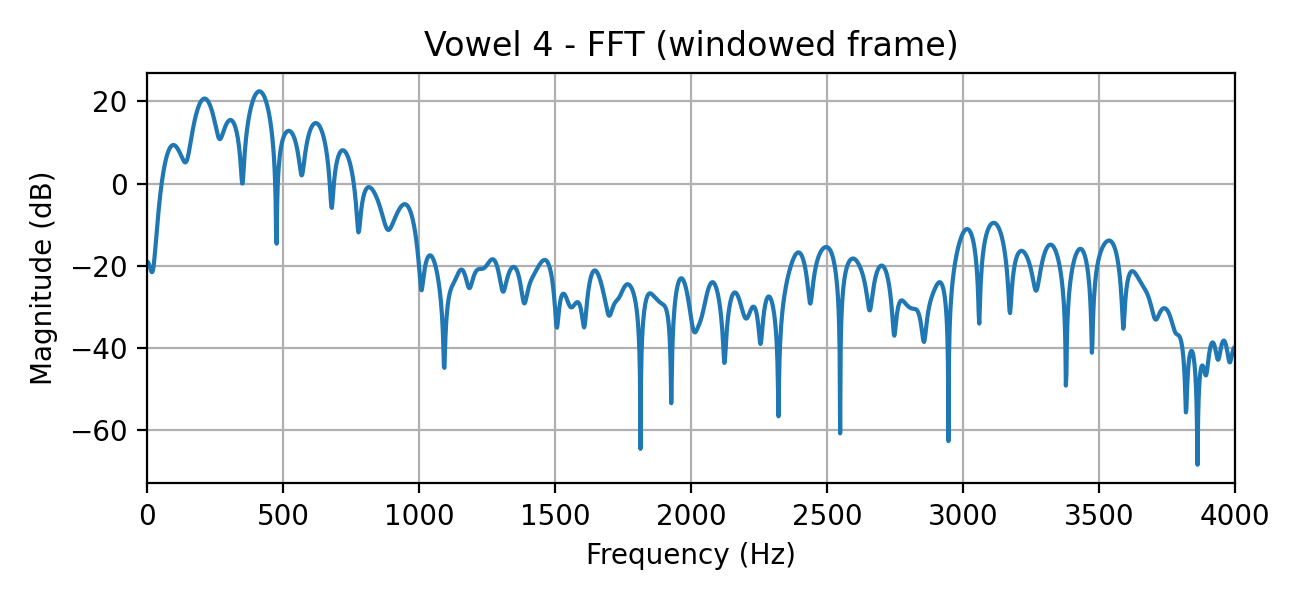
\includegraphics[width=0.9\textwidth]{vowel_report_images/vowel4_fft.png}
\subsection*{Vowel 5}
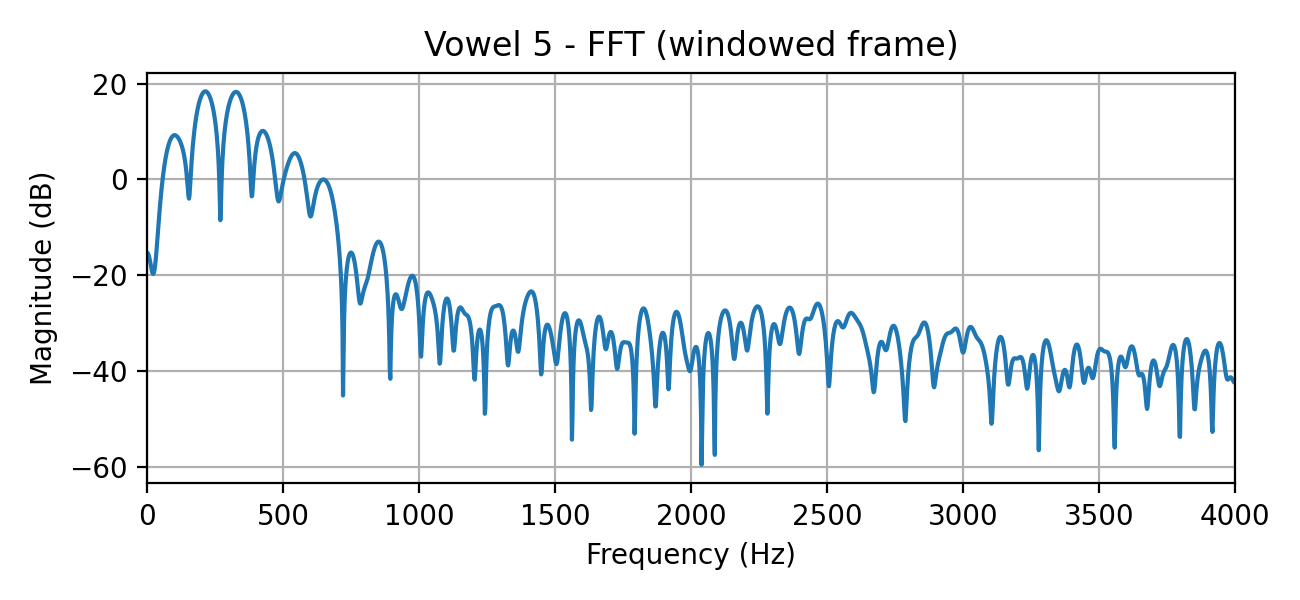
\includegraphics[width=0.9\textwidth]{vowel_report_images/vowel5_fft.png}
\section*{4. 10-th order LPC parameters (frame length approx. 25 ms)}
The LPC analysis used Levinson--Durbin to estimate a 10th-order AR model (coefficients $a[0]=1, a[1],...,a[10]$). The coefficients and prediction error power for each vowel are listed below.
\usepackage{array}
\begin{longtable}{@{} l >{\raggedright\arraybackslash}p{10cm} @{} }
\textbf{Vowel} & \textbf{LPC coefficients ($a[0]=1$) and error power}\\ \hline
Vowel 1 & Error power: 0.512212\\& LPC coeffs:\\& \verb|1.000e+00, -1.017e+00, -8.083e-01, 9.462e-01, 1.166e+00| \\
& \verb|-9.411e-01, -8.146e-01, 5.466e-01, 4.349e-01, -2.161e-01| \\
& \verb|-1.097e-01|\\[4pt]
Vowel 2 & Error power: 0.153927\\& LPC coeffs:\\& \verb|1.000e+00, -8.516e-02, -1.203e+00, -5.663e-01, 3.754e-01| \\
& \verb|3.795e-01, 7.580e-01, 1.974e-01, -6.347e-01, -3.826e-01| \\
& \verb|3.341e-01|\\[4pt]
Vowel 3 & Error power: 0.0224299\\& LPC coeffs:\\& \verb|1.000e+00, -2.085e-01, -1.446e+00, -5.656e-01, 8.677e-01| \\
& \verb|5.640e-01, 7.603e-01, -2.537e-01, -9.264e-01, -2.387e-01| \\
& \verb|5.468e-01|\\[4pt]
Vowel 4 & Error power: 0.0353563\\& LPC coeffs:\\& \verb|1.000e+00, -1.580e+00, -1.368e-01, 5.720e-01, 1.197e+00| \\
& \verb|-8.699e-01, -3.025e-01, -2.877e-01, 5.698e-01, -3.994e-03| \\
& \verb|-1.002e-01|\\[4pt]
Vowel 5 & Error power: 0.00332768\\& LPC coeffs:\\& \verb|1.000e+00, -2.066e+00, 1.037e+00, -1.620e-01, 6.477e-01| \\
& \verb|-1.695e-01, -3.902e-01, 3.727e-02, 1.226e-02, 1.098e-01| \\
& \verb|-2.330e-02|\\[4pt]
\end{longtable}
\section*{5. LPC power spectra and formants (visual observation)}
Below are the LPC envelopes (1/A) plotted in dB, overlaid with the FFT for comparison. Formant estimates (F1, F2, F3) were obtained by observing the LPC envelope peaks.
\subsection*{Vowel 1}
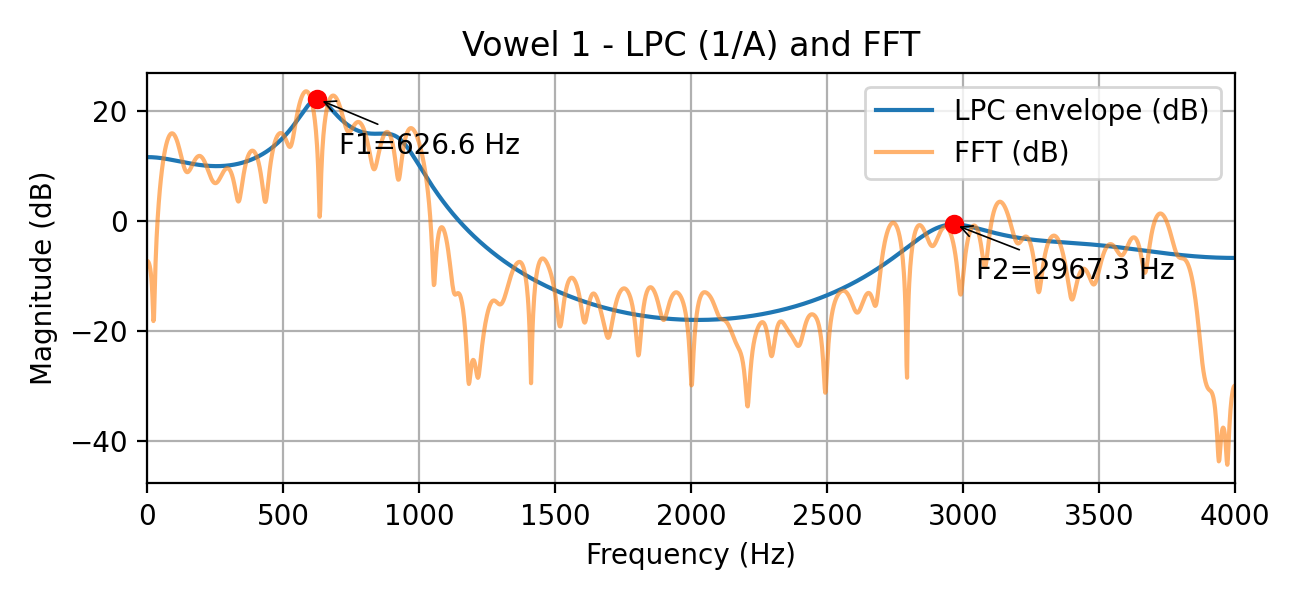
\includegraphics[width=0.9\textwidth]{vowel_report_images/vowel1_lpc.png}
\par Estimated formants: 626.6 Hz, 2967.3 Hz\\ 
\subsection*{Vowel 2}
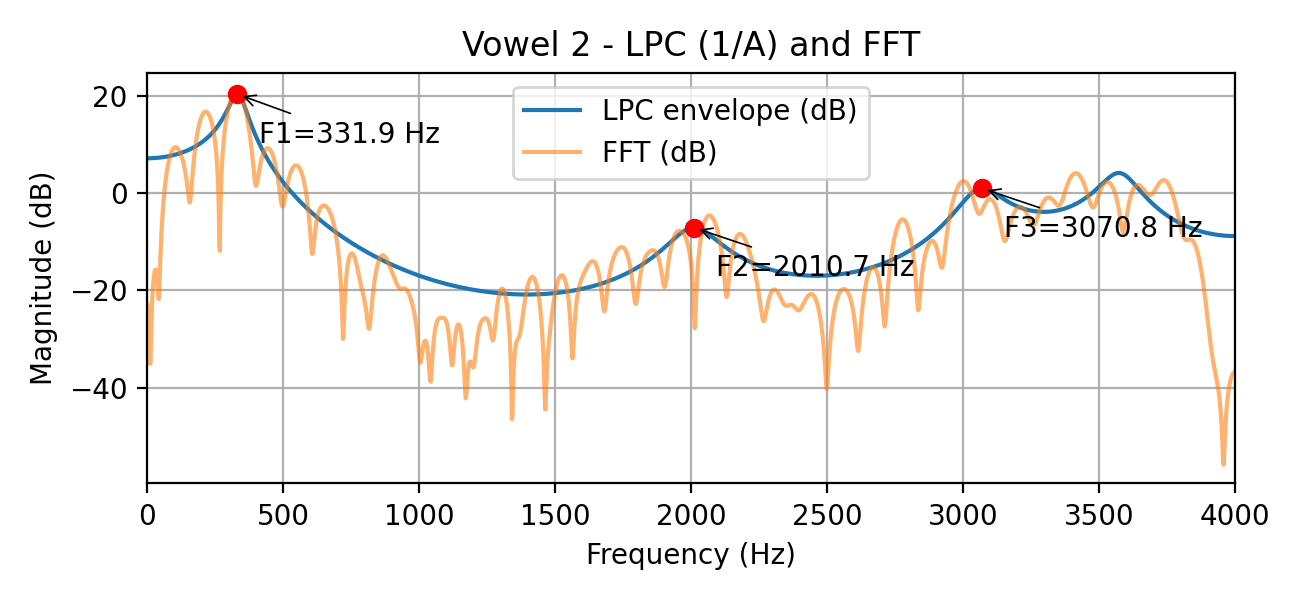
\includegraphics[width=0.9\textwidth]{vowel_report_images/vowel2_lpc.png}
\par Estimated formants: 331.9 Hz, 2010.7 Hz, 3070.8 Hz\\ 
\subsection*{Vowel 3}
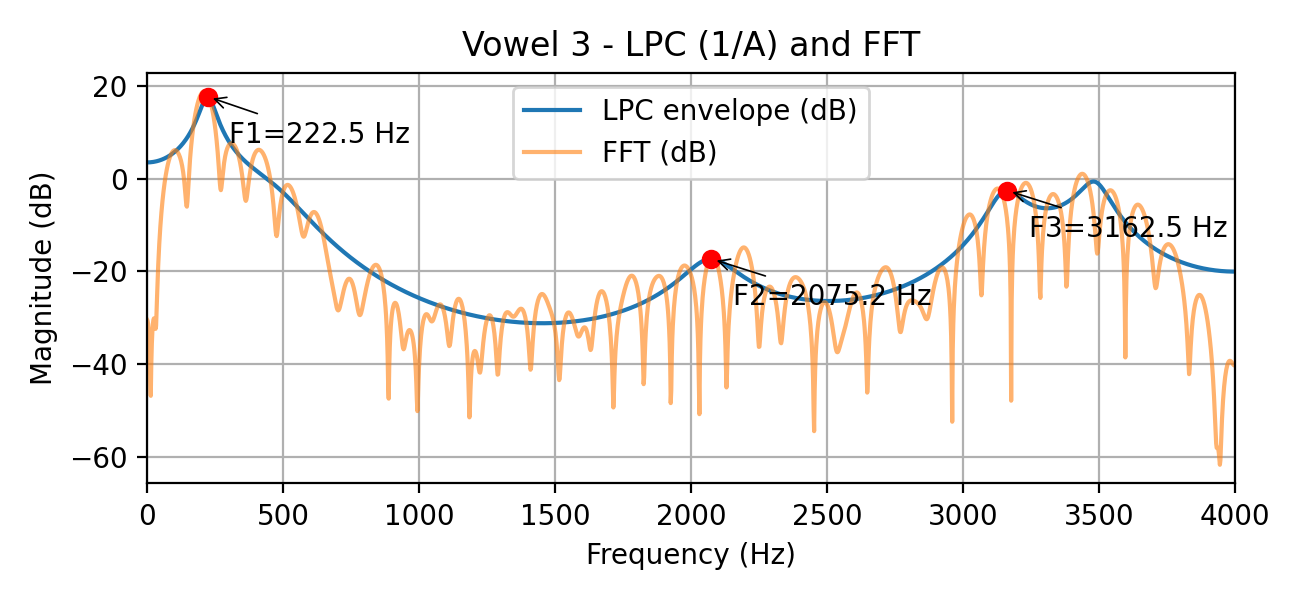
\includegraphics[width=0.9\textwidth]{vowel_report_images/vowel3_lpc.png}
\par Estimated formants: 222.5 Hz, 2075.2 Hz, 3162.5 Hz\\ 
\subsection*{Vowel 4}
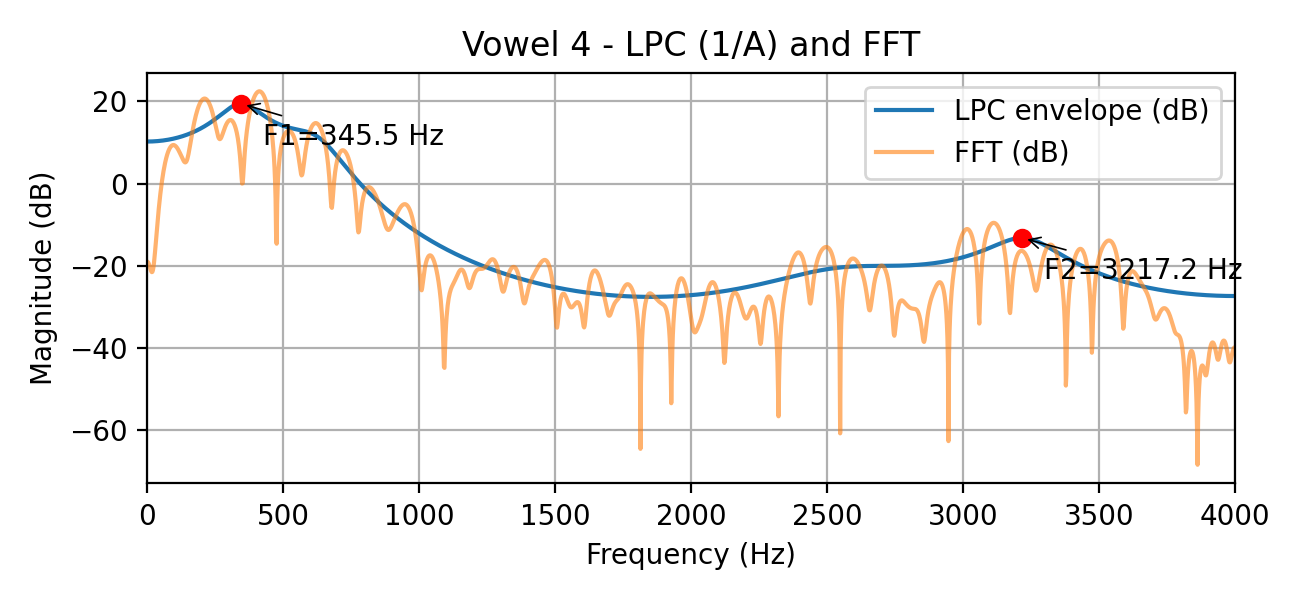
\includegraphics[width=0.9\textwidth]{vowel_report_images/vowel4_lpc.png}
\par Estimated formants: 345.5 Hz, 3217.2 Hz\\ 
\subsection*{Vowel 5}
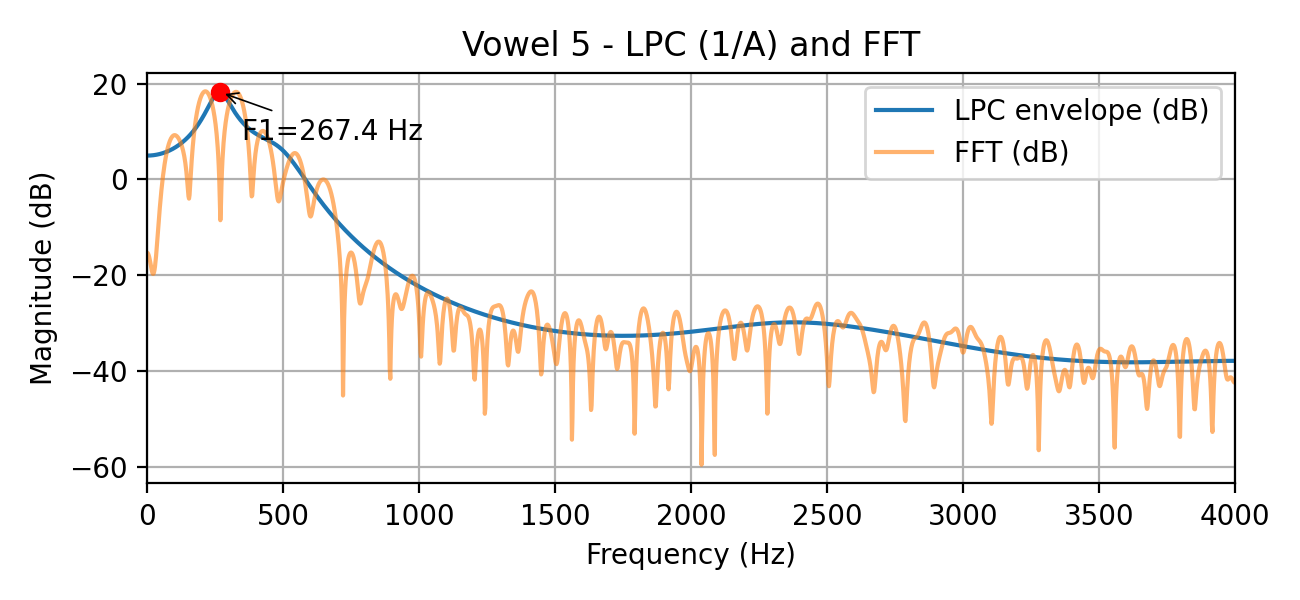
\includegraphics[width=0.9\textwidth]{vowel_report_images/vowel5_lpc.png}
\par Estimated formants: 267.4 Hz\\ 
\section*{Appendix: additional program-style graphs}
\subsection*{Autocorrelation examples and AR filter demo}
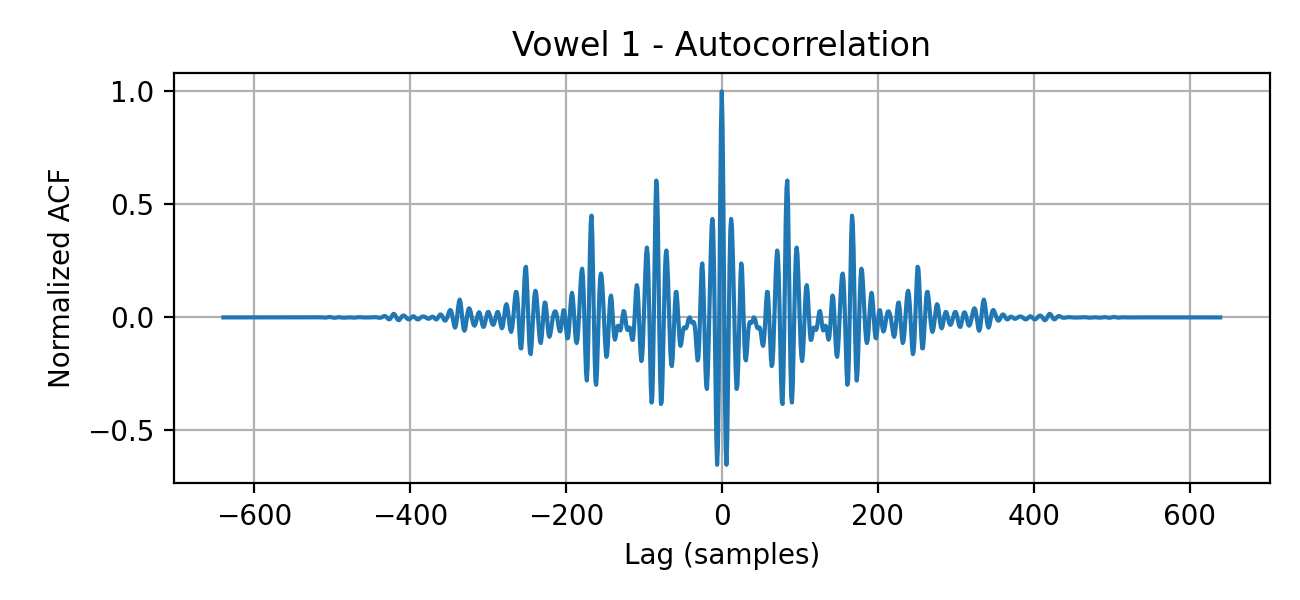
\includegraphics[width=0.9\textwidth]{vowel_report_images/vowel1_acf.png}\\
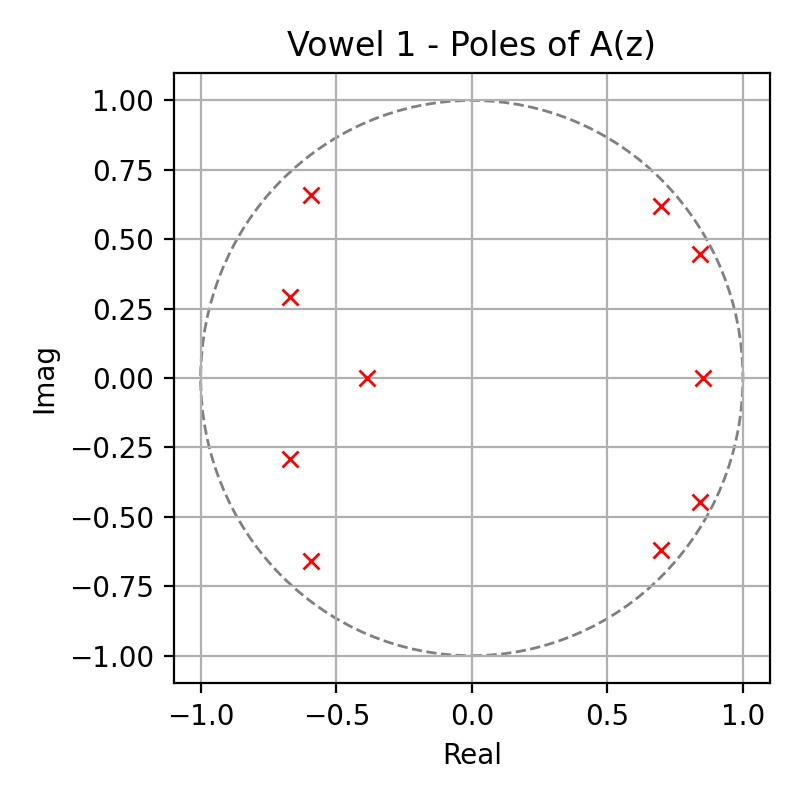
\includegraphics[width=0.9\textwidth]{vowel_report_images/vowel1_poles.png}\\
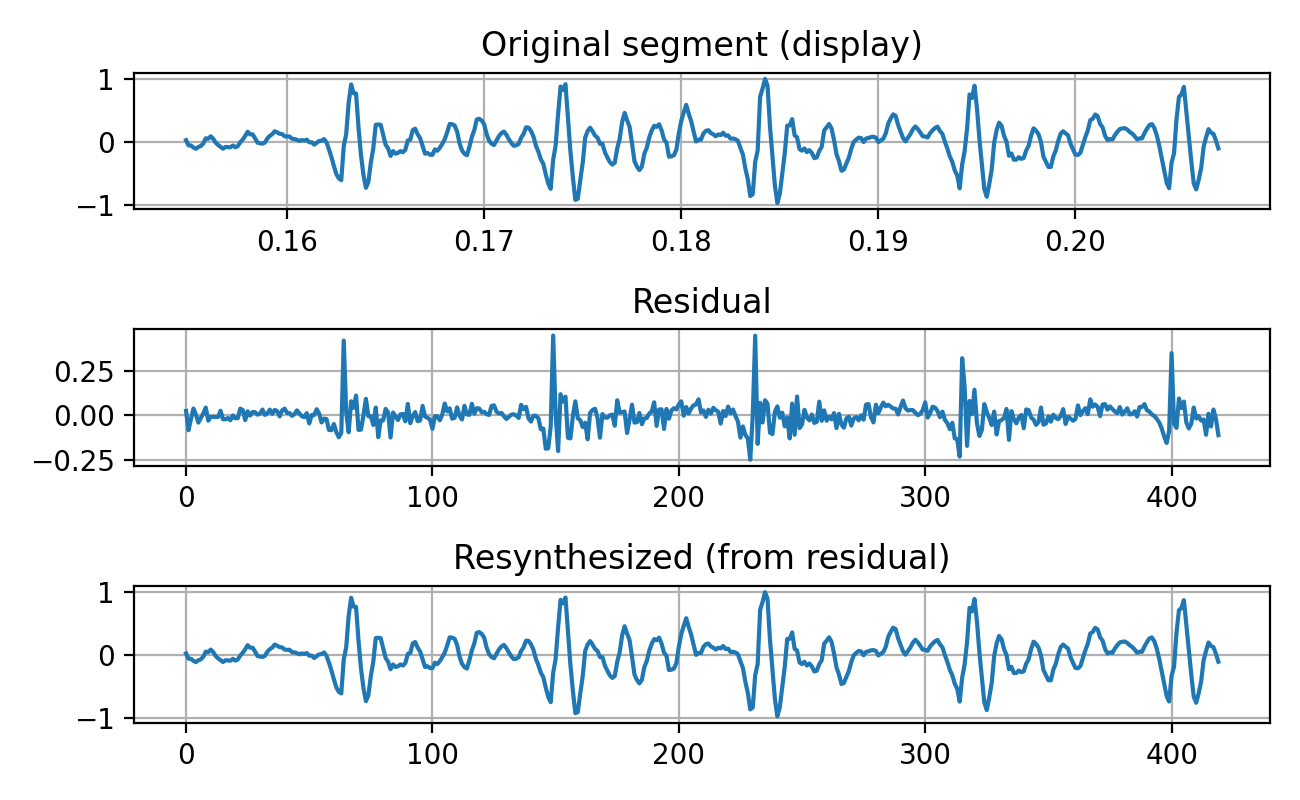
\includegraphics[width=0.9\textwidth]{vowel_report_images/vowel1_resynth.png}\\
\end{document}